\documentclass[]{article}
\usepackage{lmodern}
\usepackage{amssymb,amsmath}
\usepackage{ifxetex,ifluatex}
\usepackage{fixltx2e} % provides \textsubscript
\ifnum 0\ifxetex 1\fi\ifluatex 1\fi=0 % if pdftex
  \usepackage[T1]{fontenc}
  \usepackage[utf8]{inputenc}
\else % if luatex or xelatex
  \ifxetex
    \usepackage{mathspec}
  \else
    \usepackage{fontspec}
  \fi
  \defaultfontfeatures{Ligatures=TeX,Scale=MatchLowercase}
\fi
% use upquote if available, for straight quotes in verbatim environments
\IfFileExists{upquote.sty}{\usepackage{upquote}}{}
% use microtype if available
\IfFileExists{microtype.sty}{%
\usepackage{microtype}
\UseMicrotypeSet[protrusion]{basicmath} % disable protrusion for tt fonts
}{}
\usepackage[margin=1in]{geometry}
\usepackage{hyperref}
\hypersetup{unicode=true,
            pdftitle={R Workshop - Practice Exercises - 1.2},
            pdfborder={0 0 0},
            breaklinks=true}
\urlstyle{same}  % don't use monospace font for urls
\usepackage{color}
\usepackage{fancyvrb}
\newcommand{\VerbBar}{|}
\newcommand{\VERB}{\Verb[commandchars=\\\{\}]}
\DefineVerbatimEnvironment{Highlighting}{Verbatim}{commandchars=\\\{\}}
% Add ',fontsize=\small' for more characters per line
\usepackage{framed}
\definecolor{shadecolor}{RGB}{248,248,248}
\newenvironment{Shaded}{\begin{snugshade}}{\end{snugshade}}
\newcommand{\AlertTok}[1]{\textcolor[rgb]{0.94,0.16,0.16}{#1}}
\newcommand{\AnnotationTok}[1]{\textcolor[rgb]{0.56,0.35,0.01}{\textbf{\textit{#1}}}}
\newcommand{\AttributeTok}[1]{\textcolor[rgb]{0.77,0.63,0.00}{#1}}
\newcommand{\BaseNTok}[1]{\textcolor[rgb]{0.00,0.00,0.81}{#1}}
\newcommand{\BuiltInTok}[1]{#1}
\newcommand{\CharTok}[1]{\textcolor[rgb]{0.31,0.60,0.02}{#1}}
\newcommand{\CommentTok}[1]{\textcolor[rgb]{0.56,0.35,0.01}{\textit{#1}}}
\newcommand{\CommentVarTok}[1]{\textcolor[rgb]{0.56,0.35,0.01}{\textbf{\textit{#1}}}}
\newcommand{\ConstantTok}[1]{\textcolor[rgb]{0.00,0.00,0.00}{#1}}
\newcommand{\ControlFlowTok}[1]{\textcolor[rgb]{0.13,0.29,0.53}{\textbf{#1}}}
\newcommand{\DataTypeTok}[1]{\textcolor[rgb]{0.13,0.29,0.53}{#1}}
\newcommand{\DecValTok}[1]{\textcolor[rgb]{0.00,0.00,0.81}{#1}}
\newcommand{\DocumentationTok}[1]{\textcolor[rgb]{0.56,0.35,0.01}{\textbf{\textit{#1}}}}
\newcommand{\ErrorTok}[1]{\textcolor[rgb]{0.64,0.00,0.00}{\textbf{#1}}}
\newcommand{\ExtensionTok}[1]{#1}
\newcommand{\FloatTok}[1]{\textcolor[rgb]{0.00,0.00,0.81}{#1}}
\newcommand{\FunctionTok}[1]{\textcolor[rgb]{0.00,0.00,0.00}{#1}}
\newcommand{\ImportTok}[1]{#1}
\newcommand{\InformationTok}[1]{\textcolor[rgb]{0.56,0.35,0.01}{\textbf{\textit{#1}}}}
\newcommand{\KeywordTok}[1]{\textcolor[rgb]{0.13,0.29,0.53}{\textbf{#1}}}
\newcommand{\NormalTok}[1]{#1}
\newcommand{\OperatorTok}[1]{\textcolor[rgb]{0.81,0.36,0.00}{\textbf{#1}}}
\newcommand{\OtherTok}[1]{\textcolor[rgb]{0.56,0.35,0.01}{#1}}
\newcommand{\PreprocessorTok}[1]{\textcolor[rgb]{0.56,0.35,0.01}{\textit{#1}}}
\newcommand{\RegionMarkerTok}[1]{#1}
\newcommand{\SpecialCharTok}[1]{\textcolor[rgb]{0.00,0.00,0.00}{#1}}
\newcommand{\SpecialStringTok}[1]{\textcolor[rgb]{0.31,0.60,0.02}{#1}}
\newcommand{\StringTok}[1]{\textcolor[rgb]{0.31,0.60,0.02}{#1}}
\newcommand{\VariableTok}[1]{\textcolor[rgb]{0.00,0.00,0.00}{#1}}
\newcommand{\VerbatimStringTok}[1]{\textcolor[rgb]{0.31,0.60,0.02}{#1}}
\newcommand{\WarningTok}[1]{\textcolor[rgb]{0.56,0.35,0.01}{\textbf{\textit{#1}}}}
\usepackage{graphicx,grffile}
\makeatletter
\def\maxwidth{\ifdim\Gin@nat@width>\linewidth\linewidth\else\Gin@nat@width\fi}
\def\maxheight{\ifdim\Gin@nat@height>\textheight\textheight\else\Gin@nat@height\fi}
\makeatother
% Scale images if necessary, so that they will not overflow the page
% margins by default, and it is still possible to overwrite the defaults
% using explicit options in \includegraphics[width, height, ...]{}
\setkeys{Gin}{width=\maxwidth,height=\maxheight,keepaspectratio}
\IfFileExists{parskip.sty}{%
\usepackage{parskip}
}{% else
\setlength{\parindent}{0pt}
\setlength{\parskip}{6pt plus 2pt minus 1pt}
}
\setlength{\emergencystretch}{3em}  % prevent overfull lines
\providecommand{\tightlist}{%
  \setlength{\itemsep}{0pt}\setlength{\parskip}{0pt}}
\setcounter{secnumdepth}{0}
% Redefines (sub)paragraphs to behave more like sections
\ifx\paragraph\undefined\else
\let\oldparagraph\paragraph
\renewcommand{\paragraph}[1]{\oldparagraph{#1}\mbox{}}
\fi
\ifx\subparagraph\undefined\else
\let\oldsubparagraph\subparagraph
\renewcommand{\subparagraph}[1]{\oldsubparagraph{#1}\mbox{}}
\fi

%%% Use protect on footnotes to avoid problems with footnotes in titles
\let\rmarkdownfootnote\footnote%
\def\footnote{\protect\rmarkdownfootnote}

%%% Change title format to be more compact
\usepackage{titling}

% Create subtitle command for use in maketitle
\providecommand{\subtitle}[1]{
  \posttitle{
    \begin{center}\large#1\end{center}
    }
}

\setlength{\droptitle}{-2em}

  \title{R Workshop - Practice Exercises - 1.2}
    \pretitle{\vspace{\droptitle}\centering\huge}
  \posttitle{\par}
    \author{}
    \preauthor{}\postauthor{}
    \date{}
    \predate{}\postdate{}
  

\begin{document}
\maketitle

\hypertarget{setup}{%
\subsection{Setup}\label{setup}}

\begin{Shaded}
\begin{Highlighting}[]
\KeywordTok{library}\NormalTok{(tidyverse)}
\end{Highlighting}
\end{Shaded}

\hypertarget{the-data}{%
\subsection{The Data}\label{the-data}}

\begin{verbatim}
## Parsed with column specification:
## cols(
##   name = col_character(),
##   mfr = col_character(),
##   type = col_character(),
##   calories = col_double(),
##   protein = col_double(),
##   fat = col_double(),
##   sodium = col_double(),
##   fiber = col_double(),
##   carbo = col_double(),
##   sugars = col_double(),
##   potass = col_double(),
##   vitamins = col_double(),
##   shelf = col_double(),
##   weight = col_double(),
##   cups = col_double(),
##   rating = col_double()
## )
\end{verbatim}

\begin{Shaded}
\begin{Highlighting}[]
\NormalTok{cereals <-}\StringTok{ }\KeywordTok{read_csv}\NormalTok{(}\StringTok{"/data/cereals.csv"}\NormalTok{)}
\end{Highlighting}
\end{Shaded}

Documentation for dataset:
\url{https://www.kaggle.com/crawford/80-cereals/version/2}

\begin{Shaded}
\begin{Highlighting}[]
\CommentTok{#### Edit this code to examine your dataset}
\KeywordTok{str}\NormalTok{(cereals)}
\end{Highlighting}
\end{Shaded}

\begin{verbatim}
## Classes 'spec_tbl_df', 'tbl_df', 'tbl' and 'data.frame': 77 obs. of  16 variables:
##  $ name    : chr  "100% Bran" "100% Natural Bran" "All-Bran" "All-Bran with Extra Fiber" ...
##  $ mfr     : chr  "N" "Q" "K" "K" ...
##  $ type    : chr  "C" "C" "C" "C" ...
##  $ calories: num  70 120 70 50 110 110 110 130 90 90 ...
##  $ protein : num  4 3 4 4 2 2 2 3 2 3 ...
##  $ fat     : num  1 5 1 0 2 2 0 2 1 0 ...
##  $ sodium  : num  130 15 260 140 200 180 125 210 200 210 ...
##  $ fiber   : num  10 2 9 14 1 1.5 1 2 4 5 ...
##  $ carbo   : num  5 8 7 8 14 10.5 11 18 15 13 ...
##  $ sugars  : num  6 8 5 0 8 10 14 8 6 5 ...
##  $ potass  : num  280 135 320 330 -1 70 30 100 125 190 ...
##  $ vitamins: num  25 0 25 25 25 25 25 25 25 25 ...
##  $ shelf   : num  3 3 3 3 3 1 2 3 1 3 ...
##  $ weight  : num  1 1 1 1 1 1 1 1.33 1 1 ...
##  $ cups    : num  0.33 1 0.33 0.5 0.75 0.75 1 0.75 0.67 0.67 ...
##  $ rating  : num  68.4 34 59.4 93.7 34.4 ...
##  - attr(*, "spec")=
##   .. cols(
##   ..   name = col_character(),
##   ..   mfr = col_character(),
##   ..   type = col_character(),
##   ..   calories = col_double(),
##   ..   protein = col_double(),
##   ..   fat = col_double(),
##   ..   sodium = col_double(),
##   ..   fiber = col_double(),
##   ..   carbo = col_double(),
##   ..   sugars = col_double(),
##   ..   potass = col_double(),
##   ..   vitamins = col_double(),
##   ..   shelf = col_double(),
##   ..   weight = col_double(),
##   ..   cups = col_double(),
##   ..   rating = col_double()
##   .. )
\end{verbatim}

\begin{Shaded}
\begin{Highlighting}[]
\KeywordTok{summary}\NormalTok{(cereals)}
\end{Highlighting}
\end{Shaded}

\begin{verbatim}
##      name               mfr                type              calories    
##  Length:77          Length:77          Length:77          Min.   : 50.0  
##  Class :character   Class :character   Class :character   1st Qu.:100.0  
##  Mode  :character   Mode  :character   Mode  :character   Median :110.0  
##                                                           Mean   :106.9  
##                                                           3rd Qu.:110.0  
##                                                           Max.   :160.0  
##     protein           fat            sodium          fiber       
##  Min.   :1.000   Min.   :0.000   Min.   :  0.0   Min.   : 0.000  
##  1st Qu.:2.000   1st Qu.:0.000   1st Qu.:130.0   1st Qu.: 1.000  
##  Median :3.000   Median :1.000   Median :180.0   Median : 2.000  
##  Mean   :2.545   Mean   :1.013   Mean   :159.7   Mean   : 2.152  
##  3rd Qu.:3.000   3rd Qu.:2.000   3rd Qu.:210.0   3rd Qu.: 3.000  
##  Max.   :6.000   Max.   :5.000   Max.   :320.0   Max.   :14.000  
##      carbo          sugars           potass          vitamins     
##  Min.   :-1.0   Min.   :-1.000   Min.   : -1.00   Min.   :  0.00  
##  1st Qu.:12.0   1st Qu.: 3.000   1st Qu.: 40.00   1st Qu.: 25.00  
##  Median :14.0   Median : 7.000   Median : 90.00   Median : 25.00  
##  Mean   :14.6   Mean   : 6.922   Mean   : 96.08   Mean   : 28.25  
##  3rd Qu.:17.0   3rd Qu.:11.000   3rd Qu.:120.00   3rd Qu.: 25.00  
##  Max.   :23.0   Max.   :15.000   Max.   :330.00   Max.   :100.00  
##      shelf           weight          cups           rating     
##  Min.   :1.000   Min.   :0.50   Min.   :0.250   Min.   :18.04  
##  1st Qu.:1.000   1st Qu.:1.00   1st Qu.:0.670   1st Qu.:33.17  
##  Median :2.000   Median :1.00   Median :0.750   Median :40.40  
##  Mean   :2.208   Mean   :1.03   Mean   :0.821   Mean   :42.67  
##  3rd Qu.:3.000   3rd Qu.:1.00   3rd Qu.:1.000   3rd Qu.:50.83  
##  Max.   :3.000   Max.   :1.50   Max.   :1.500   Max.   :93.70
\end{verbatim}

{[}Briefly summarize the dataset here.{]}

{[}CHECKPOINT: Knit your Markdown file!{]}

\hypertarget{data-cleaning-and-transformation}{%
\subsection{Data Cleaning and
Transformation}\label{data-cleaning-and-transformation}}

\begin{Shaded}
\begin{Highlighting}[]
\NormalTok{cereals }\OperatorTok
\StringTok{  }\KeywordTok{summarize_at}\NormalTok{(}\KeywordTok{vars}\NormalTok{(calories, sugars),}
            \KeywordTok{funs}\NormalTok{(mean, median))}
\end{Highlighting}
\end{Shaded}

\begin{verbatim}
## # A tibble: 1 x 4
##   calories_mean sugars_mean calories_median sugars_median
##           <dbl>       <dbl>           <dbl>         <dbl>
## 1          107.        6.92             110             7
\end{verbatim}

\begin{Shaded}
\begin{Highlighting}[]
\NormalTok{cereals_}\DecValTok{2}\NormalTok{ <-}\StringTok{ }\NormalTok{cereals }\OperatorTok
\StringTok{  }\KeywordTok{mutate}\NormalTok{(}
    \DataTypeTok{cal_per_cup =}\NormalTok{ calories}\OperatorTok{/}\NormalTok{cups}
\NormalTok{  ) }\OperatorTok
\StringTok{  }\KeywordTok{select}\NormalTok{(name, mfr, cal_per_cup) }\OperatorTok
\StringTok{  }\KeywordTok{filter}\NormalTok{(mfr }\OperatorTok{==}\StringTok{ "Kellogg"}\NormalTok{) }\OperatorTok
\StringTok{  }\KeywordTok{arrange}\NormalTok{(cal_per_cup)}
\end{Highlighting}
\end{Shaded}

{[}CHECKPOINT: Knit your document!{]}

\hypertarget{visualizing-the-data}{%
\subsection{Visualizing the data}\label{visualizing-the-data}}

\hypertarget{histogram}{%
\subsubsection{Histogram}\label{histogram}}

\begin{Shaded}
\begin{Highlighting}[]
\KeywordTok{ggplot}\NormalTok{(cereals, }\KeywordTok{aes}\NormalTok{(}\DataTypeTok{x =}\NormalTok{ sugars)) }\OperatorTok{+}\StringTok{ }
\StringTok{  }\KeywordTok{geom_histogram}\NormalTok{(}\DataTypeTok{bins =} \DecValTok{10}\NormalTok{, }\DataTypeTok{fill =} \StringTok{"cornflowerblue"}\NormalTok{) }\OperatorTok{+}
\StringTok{  }\KeywordTok{ggtitle}\NormalTok{(}\StringTok{"Sugar content of cereals"}\NormalTok{)}
\end{Highlighting}
\end{Shaded}

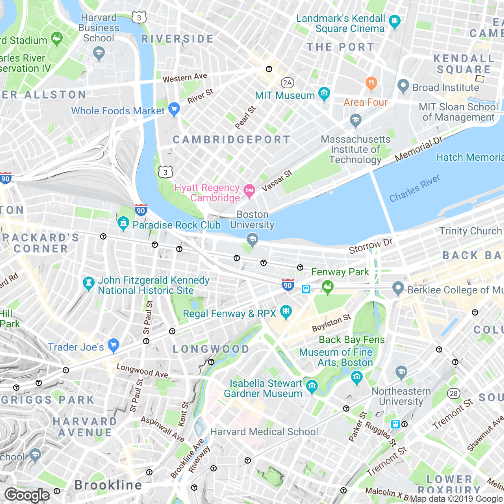
\includegraphics{Activity-soln_files/figure-latex/unnamed-chunk-7-1.pdf}

\hypertarget{bar-plot}{%
\subsubsection{Bar Plot}\label{bar-plot}}

\begin{Shaded}
\begin{Highlighting}[]
\KeywordTok{ggplot}\NormalTok{(cereals, }\KeywordTok{aes}\NormalTok{(}\DataTypeTok{x =}\NormalTok{ mfr, }\DataTypeTok{fill =}\NormalTok{ mfr)) }\OperatorTok{+}\StringTok{ }
\StringTok{  }\KeywordTok{geom_bar}\NormalTok{() }\OperatorTok{+}
\StringTok{  }\KeywordTok{ggtitle}\NormalTok{(}\StringTok{"Manufacturers"}\NormalTok{)}
\end{Highlighting}
\end{Shaded}

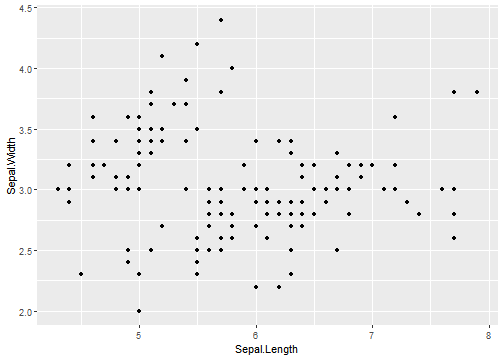
\includegraphics{Activity-soln_files/figure-latex/unnamed-chunk-8-1.pdf}

\hypertarget{box-plot}{%
\subsubsection{Box Plot}\label{box-plot}}

\begin{Shaded}
\begin{Highlighting}[]
\KeywordTok{ggplot}\NormalTok{(cereals, }\KeywordTok{aes}\NormalTok{(}\DataTypeTok{x =}\NormalTok{ mfr, }\DataTypeTok{y =}\NormalTok{ sugars, }\DataTypeTok{fill =}\NormalTok{ mfr)) }\OperatorTok{+}\StringTok{ }
\StringTok{  }\KeywordTok{geom_boxplot}\NormalTok{() }\OperatorTok{+}
\StringTok{  }\KeywordTok{ggtitle}\NormalTok{(}\StringTok{"Sugar content of cereals by manufacturer"}\NormalTok{)}
\end{Highlighting}
\end{Shaded}

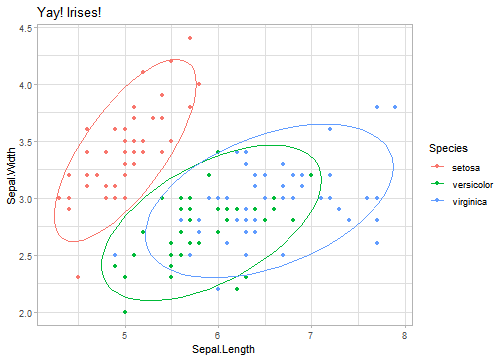
\includegraphics{Activity-soln_files/figure-latex/unnamed-chunk-9-1.pdf}

\hypertarget{scatter-plot}{%
\subsubsection{Scatter Plot}\label{scatter-plot}}

\begin{Shaded}
\begin{Highlighting}[]
\KeywordTok{ggplot}\NormalTok{(cereals, }\KeywordTok{aes}\NormalTok{(}\DataTypeTok{x =}\NormalTok{ sugars, }\DataTypeTok{y =}\NormalTok{ calories)) }\OperatorTok{+}\StringTok{ }
\StringTok{  }\KeywordTok{geom_point}\NormalTok{() }\OperatorTok{+}
\StringTok{  }\KeywordTok{ggtitle}\NormalTok{(}\StringTok{"Sugar and calorie content of cereals"}\NormalTok{)}
\end{Highlighting}
\end{Shaded}

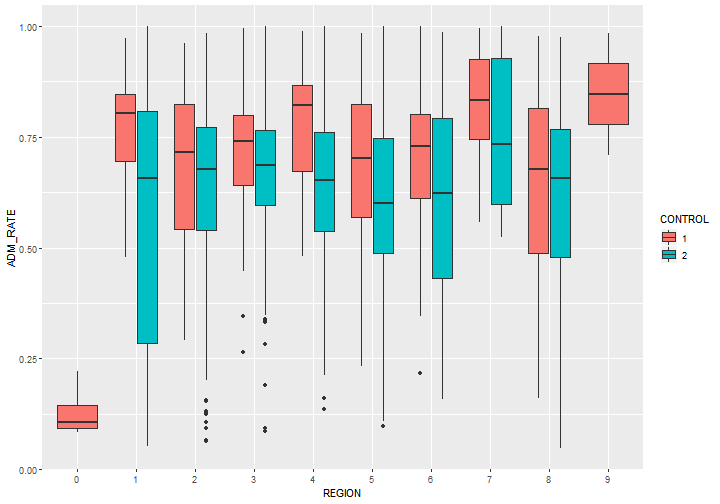
\includegraphics{Activity-soln_files/figure-latex/unnamed-chunk-10-1.pdf}

\hypertarget{conclusion}{%
\subsection{Conclusion}\label{conclusion}}

What did you learn about cereals? Write a few sentences summarizing your
findings, knit your document, and admire your handiwork!


\end{document}
